\documentclass[cn, hazy, blue, normal, 12pt]{elegantnote}

\title{组合数学例题讲解}
\author{Mobyw}
\version{1.0}
\date{\zhtoday}

\usepackage{tikz}
\usepackage{pgfplots}
\usepackage{bookmark}
\usepackage{multirow}
\usepackage{tabularx}
\usepackage[verbose]{xsim}
\usepackage[enableskew,vcentermath]{youngtab}

\usetikzlibrary{patterns}
\pgfplotsset{compat=1.18}

\tikzset{
    box/.style ={
        rectangle,              % 矩形节点
        rounded corners = 5pt,  % 圆角
        minimum width   = 50pt, % 最小宽度
        minimum height  = 20pt, % 最小高度
        inner sep = 5pt,        % 文字和边框的距离
        draw=blue               % 边框颜色
    }
}

\begin{document}

\maketitle

% \setlength{\lineskip}{1.5em}
% \setlength{\parskip}{0pt}


本文为组合数学各章节的例题,由于部分答案为个人编撰,难免会出现错误,请保证使用 \href{https://github.com/mobyw/MasterCourseNotes/blob/master/CombinatorialMathematics/CombinatorialMathematicsExamples.pdf}{GitHub仓库} 所发布的最新版本. 如遇问题可在 GitHub 上发布 Issue.


\section{容斥原理}

\begin{exercise}

    求方程:
    \begin{equation}
        \notag
        \left\{\begin{array}{l}
            x_{1}+x_{2}+x_{3}+x_{4}=13 \\
            3 \leq x_{1} \leq 6, 2 \leq x_{2} \leq 6, x_{3} \leq 2
        \end{array}\right.
    \end{equation}

    正整数解的个数.

\end{exercise}

\begin{solution}[print=true]

    首先进行变量代换:
    \begin{equation}
        \notag
        x_1^{\prime} = x_1-3,
        x_2^{\prime} = x_2-2,
        x_3^{\prime} = x_3-1,
        x_4^{\prime} = x_4-1
    \end{equation}

    则方程变为:
    \begin{equation}
        \notag
        \left\{
        \begin{array}{l}
            x_1^{\prime} + x_2^{\prime} + x_3^{\prime} + x_4^{\prime} = 6 \\
            0 \leq x_1^{\prime} \leq 3,
            0 \leq x_2^{\prime} \leq 4,
            0 \leq x_3^{\prime} \leq 1,
            x_4^{\prime} \geq 0
        \end{array}
        \right.
    \end{equation}

    等价为求集合 $S_0$ 的 $6\text{-}$组合数,其中 $S_0$ 为:
    \begin{equation}
        \notag
        S_0 = \left\{
        3 \cdot x_1^{\prime},
        4 \cdot x_2^{\prime},
        1 \cdot x_3^{\prime},
        \infty \cdot x_4^{\prime}
        \right\}
    \end{equation}

    用 $A_1$ 表示 $S$ 中至少含有 $4$ 个 $x_1^{\prime}$;$A_2$ 表示 $S$ 中至少含有 $5$ 个 $x_2^{\prime}$;$A_3$ 表示 $S$ 中至少含有 $2$ 个 $x_3^{\prime}$. 其中 $S$ 为:
    \begin{equation}
        \notag
        S = \left\{
        \infty \cdot x_1^{\prime},
        \infty \cdot x_2^{\prime},
        \infty \cdot x_3^{\prime},
        \infty \cdot x_4^{\prime}
        \right\}
    \end{equation}

    根据容斥原理,所求的 $6\text{-}$组合数为:
    \begin{equation}
        \notag
        \begin{aligned}
              & \left| \overline{A}_1 \cap
            \overline{A}_2 \cap
            \overline{A}_3 \right|                         \\
            = & |S| -
            \sum_{i=1}^{3}{\left| A_i \right|} +
            \sum_{i \neq j}{\left| A_i \cap A_j \right|} -
            \left| A_1 \cap A_2 \cap A_3 \right|           \\
            = & F(4,6) -
            \left(F(4,2)+F(4,1)+F(4,4)\right) + F(4,0) - 0 \\
            = & 84-(10+4+35)+1                             \\
            = & 36
        \end{aligned}
    \end{equation}

    故原方程的正整数解个数为 $36$.

\end{solution}

\begin{exercise}

    奔赴抗疫,全国 $4$ 个片区共有 $68$ 个医疗队,其中西南片区有 $10$ 个,中部片区有 $18$ 个,北方片区有 $18$ 个,东部片区有 $22$ 个. 假定同一片区的各个医疗队不加以区别,现在要从中选取 $27$ 个医疗队入围. 考虑到不同片区的特殊情况,要求西南片区至少入围 $4$ 个医疗队,北方片区至少入围 $7$ 个医疗队,其他片区至少各入围 $2$ 个医疗队,问理论上有多少种不同的选取方案?

\end{exercise}

\begin{solution}[print=true]

    用 $x_{1}, x_{2}, x_{3}, x_{4}$ 表示四个片区的选取数目,则有:
    \begin{equation}
        \notag
        \left\{\begin{array}{l}
            x_{1}+x_{2}+x_{3}+x_{4}=27 \\
            4 \leq x_1 \leq 10,
            2 \leq x_2 \leq 18,
            7 \leq x_3 \leq 18,
            2 \leq x_4 \leq 22
        \end{array}\right.
    \end{equation}

\end{solution}

\begin{exercise}

    有数学、物理、化学和英语 $4$ 门课程. 现从星期一到星期四安排这四门课程,每门课程安排一天,每天安排一门课程. 要求数学不能安排在星期一和星期二,物理不能安排在星期三,化学不能安排在星期四,英语不能安排在星期二. 问有多少种不同的安排方案?

\end{exercise}

\begin{solution}[print=true]

    禁区棋盘:

    \begin{center}
        \notag
        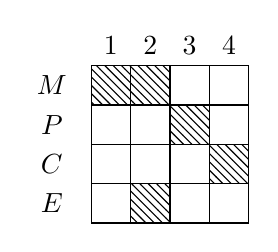
\begin{tikzpicture}[scale=.5,line width=0.5pt]
            \node at(-1,3.5) {$M$};
            \node at(-1,2.5) {$P$};
            \node at(-1,1.5) {$C$};
            \node at(-1,0.5) {$E$};

            \node at(0.5,4.5) {$1$};
            \node at(1.5,4.5) {$2$};
            \node at(2.5,4.5) {$3$};
            \node at(3.5,4.5) {$4$};

            \filldraw[pattern=north west lines] (0,3) rectangle (1,4);
            \filldraw[pattern=north west lines] (1,3) rectangle (2,4);
            \draw (2,3) rectangle (3,4);
            \draw (3,3) rectangle (4,4);

            \draw (0,2) rectangle (1,3);
            \draw (1,2) rectangle (2,3);
            \filldraw[pattern=north west lines] (2,2) rectangle (3,3);
            \draw (3,2) rectangle (4,3);

            \draw (0,1) rectangle (1,2);
            \draw (1,1) rectangle (2,2);
            \draw (2,1) rectangle (3,2);
            \filldraw[pattern=north west lines] (3,1) rectangle (4,2);

            \draw (0,0) rectangle (1,1);
            \filldraw[pattern=north west lines] (1,0) rectangle (2,1);
            \draw (2,0) rectangle (3,1);
            \draw (3,0) rectangle (4,1);
        \end{tikzpicture}
    \end{center}

    禁区棋盘计算:
    \begin{equation}
        \notag
        \begin{aligned}
            R \left(\young(~~::,::~:,:::~,:~::)\right)
             & = x R \left(\young(~:,:~)\right)+
            R \left(\young(~:::,::~:,:::~,:~::)\right)              \\
             & = x R \left(\young(~:,:~)\right)+
            R^2 \left(\young(~)\right) R \left(\young(~:,:~)\right) \\
             & = x(1+2x+x^2) + (1+x)^2(1+2x+x^2)                    \\
             & =1+5x+8x^2+5x^3+x^4
        \end{aligned}
    \end{equation}

    安排方案数:
    \begin{equation}
        \notag
        N = 4! - 5 \cdot 3! + 8 \cdot 2! - 5 + 1 = 6
    \end{equation}

\end{solution}


\section{鸽笼原理与 Ramsey 定理}

\begin{exercise}

    证明 $11$ 个人中必定有 $4$ 个人彼此相认或 $3$ 个人彼此不相识.

\end{exercise}

\begin{solution}[print=true]

    在这 $11$ 个人中任意挑选一个人 $p$,则剩下的 $10$ 个人可以分成两个集合 $F$ 和 $S$,其中 $F$ 表示与 $p$ 相识的人的集合;$S$ 表示与 $p$ 不相识的人的集合.

    如果 $S$ 中有 $4$ 个及以上人,则这些人可能彼此相识或者至少有两个人彼此不相识. 第一种情况中有 $4$ 个人彼此相识,命题成立;第二种情况中有两人彼此不相识,则这两个人也与 $p$ 不相识,于是有 $3$ 个人彼此不相识,命题成立.

    如果在 $S$ 中最多有 $3$ 个人,则 $F$ 中至少有 $7$ 个人.

    在 $F$ 的 $7$ 个人中任意挑选一个人 $q$,则剩下的 $6$ 个人可以分成两个集合 $G$ 和 $T$,其中 $G$ 表示与 $q$ 相识的人的集合;$T$ 表示与 $q$ 不相识的人的集合. 由鸽笼原理知,$G$ 和 $T$ 至少有一个有 $3$ 个及以上人.

    如果 $T$ 中有 $3$ 个及以上人,则这些人可能彼此相识或者至少有两个人彼此不相识. 第一种情况中有 $3$ 个人彼此相识,同时也与 $p$ 相识,于是有 $4$ 个人彼此相识,命题成立;第二种情况中有两人彼此不相识,则这两个人也与 $q$ 不相识,于是有 $3$ 个人彼此不相识,命题成立.

    如果 $G$ 中有 $3$ 个及以上人,则这些人可能彼此不相识或者至少有两个人彼此相识. 第一种情况中有 $3$ 个人彼此不相识,命题成立;第二种情况中有两人彼此相识,则这两个人也与 $q$ 和 $p$ 相识,于是有 $4$ 个人彼此相识,命题成立.

\end{solution}

\begin{exercise}

    证明 $R(3, 3) < 7$.

\end{exercise}

\begin{solution}[print=true]

    根据公式:
    \begin{equation}
        \notag
        \begin{array}{c}
            R(a, b) \leq R(a-1, b)+R(a, b-1) \\
            R(a, b) = R(b, a)                \\
            R(a, 2) = a
        \end{array}
    \end{equation}

    可得:
    \begin{equation}
        \notag
        \begin{array}{c}
            R(3, 3) \leq R(2, 3) + R(3, 2) = 2 R(3, 2) = 2 \cdot 3 = 6 \\
            R(3, 3) \leq 6                                             \\
            R(3, 3) < 7
        \end{array}
    \end{equation}

\end{solution}


\section{母函数}

\begin{exercise}

    求方程:
    \begin{equation}
        \notag
        \left\{\begin{array}{l}
            x_{1}+3 x_{2}+x_{3}+x_{4}=160 \\
            3 \leq x_{2} \leq 10, x_{3} \leq 3
        \end{array}\right.
    \end{equation}

    正整数解的个数.

\end{exercise}

\begin{solution}[print=true]

    首先进行变量代换:
    \begin{equation}
        \notag
        x_1^{\prime} = x_1-1,
        x_2^{\prime} = x_2-3,
        x_3^{\prime} = x_3-1,
        x_4^{\prime} = x_4-1
    \end{equation}

    则方程变为:
    \begin{equation}
        \notag
        \left\{
        \begin{array}{l}
            x_1^{\prime} + 3 x_2^{\prime} + x_3^{\prime} + x_4^{\prime} = 148 \\
            x_1^{\prime} \geq 0,
            0 \leq x_2^{\prime} \leq 7,
            0 \leq x_3^{\prime} \leq 2,
            x_4^{\prime} \geq 0
        \end{array}
        \right.
    \end{equation}

    其母函数为:
    \begin{equation}
        \notag
        \begin{aligned}
            f(x) & = (1+x+x^2+\cdots)^2
            (1+x^3+x^6+\cdots+x^{21})
            (1+x+x^2)                            \\
                 & = \dfrac{1}{(1-x)^2} \cdot
            \dfrac{1-x^{24}}{1-x^3} \cdot
            \dfrac{1-x^3}{1-x}                   \\
                 & = \dfrac{1-x^{24}}{(1-x)^3}   \\
                 & = \left(1-x^{24}\right) \cdot
            \sum_{k=0}^{\infty} {\left(
                \begin{array}{c} 2+k \\ 2 \end{array}
                \right) x^k}
        \end{aligned}
    \end{equation}

    其中 $x$ 系数是 $148$ 的对应 $k=148$ 和 $k=148-24=124$ 两种取值:
    \begin{equation}
        \notag
        \begin{aligned}
            a_{148}
             & = \left(
            \begin{array}{c} 2+148 \\ 2 \end{array}
            \right) -
            \left(
            \begin{array}{c} 2+124 \\ 2 \end{array}
            \right)     \\
             & = 3300
        \end{aligned}
    \end{equation}

    故原方程的正整数解个数为 $3300$.

\end{solution}

\begin{exercise}

    求方程:
    \begin{equation}
        \notag
        \left\{\begin{array}{l}
            x_{1}+x_{2}+4 x_{3}+x_{4}=160 \\
            2 \leq x_{3} \leq 10, x_{4} \leq 3
        \end{array}\right.
    \end{equation}

    正整数解的个数.

\end{exercise}

\begin{exercise}

    求不包含 $3, 5, 7$,出现偶数次 $1, 2$,至少出现两次 $4, 8$ 的 $r$ 位十进制数的个数.

\end{exercise}

\begin{solution}[print=true]

    设 $a_r$ 是由 $0, 1, 2, 4, 6, 8, 9$ 组成的有偶数个 $1, 2$,至少两个 $4, 8$ ,长度为 $r$ 的序列.

    则 $a_r$ 的指数母函数为:
    \begin{equation}
        \notag
        \begin{aligned}
            f_4(x)
             & = \left(1+\frac{x^2}{2!}+\frac{x^4}{4!}+\cdots\right)^2
            \left(\frac{x^2}{2!}+\frac{x^3}{3!}+\frac{x^4}{4!}+\cdots\right)^2
            \left(1+\frac{x}{1!}+\frac{x^2}{2!}+\cdots\right)^3                \\
             & = \left(\frac{\mathrm{e}^{x}+\mathrm{e}^{-x}}{2}\right)^2 \cdot
            \left(\mathrm{e}^{x}-1\right)^2 \cdot
            \mathrm{e}^{3x}                                                    \\
             & = \frac{1}{4}\left(
            \mathrm{e}^{7x}-2\mathrm{e}^{6x}+3\mathrm{e}^{5x}-4\mathrm{e}^{4x}+
            3\mathrm{e}^{3x}-\mathrm{e}^{2x}+\mathrm{e}^{x}
            \right)                                                            \\
             & =\sum_{r=0}^{\infty}{\frac{1}{4}\left(
            7^r - 2 \cdot 6^r + 3 \cdot 5^r - 4 \cdot 4^r+
            3 \cdot 3^r- 2 \cdot 2^r + 1
            \right)\frac{x^r}{r!}}
        \end{aligned}
    \end{equation}

    可知:
    \begin{equation}
        \notag
        a_r = \frac{1}{4}\left(
        7^r - 2 \cdot 6^r + 3 \cdot 5^r - 4 \cdot 4^r+
        3 \cdot 3^r- 2 \cdot 2^r + 1
        \right)
    \end{equation}

    首位取 $0$ 的 $r$ 位序列个数为 $a_{r-1}$,所以所求的 $r$ 位十进制数个数为:
    \begin{equation}
        \notag
        a_r - a_{r-1} = \left\{
        \begin{aligned}
             & \frac{1}{4} \cdot \left(
            6 \cdot 7^{r-1} - 10 \cdot 6^{r-1} +
            12 \cdot 5^{r-1} - 12 \cdot 4^{r-1} +
            6 \cdot 3^{r-1} - 2 \cdot 2^{r-1}
            \right)
             & , r>0                    \\
             & 0
             & , r=0
        \end{aligned}
        \right.
    \end{equation}

\end{solution}


\section{递归关系}

\begin{exercise}

    求解递归关系:
    \begin{equation}
        \notag
        \left\{\begin{array}{l}
            a_{n}-2 a_{n-1}-3 a_{n-2} = 2 \cdot 3^{n} \\
            a_{0}=1, a_{1}=2
        \end{array}\right.
    \end{equation}

\end{exercise}

\begin{solution}[print=true]

    对应的齐次关系的特征方程为:
    \begin{equation}
        \notag
        x^2 - 2x - 3 = 0
    \end{equation}

    齐次方程的根为:
    \begin{equation}
        \notag
        p_1 = -1, p_2 = 3
    \end{equation}

    故通解为:
    \begin{equation}
        \notag
        a_n^\ast = c_1 p_1^n + c_2 p_2^n = c_1 \cdot (-1)^n + c_2 \cdot 3^n
    \end{equation}

    又有 $f(n)=3^n$,且 $3$ 是递归关系式的特征根,故设特解为:
    \begin{equation}
        \notag
        \overline{a}_{n} = An \cdot 3^n
    \end{equation}

    带入原递归关系得:
    \begin{equation}
        \notag
        \begin{array}{c}
            An \cdot 3^{n} - 2A(n-1) \cdot
            3^{n-1} -3A(n-2) \cdot 3^{n-2} =
            2 \cdot 3^{n} \\
            A = \dfrac{3}{2}
        \end{array}
    \end{equation}

    故通解为:
    \begin{equation}
        \notag
        a_{n} =
        a_{n}^{\ast} + \overline{a}_{n}
        = c_1 \cdot (-1)^n + c_2 \cdot 3^n + \dfrac{3}{2} n \cdot 3^n
    \end{equation}

    由初始条件得:
    \begin{equation}
        \notag
        \left\{
        \begin{array}{l}
            c_{1} + c_{2} + 0 = 1 \\
            -c_{1} + 3 c_{2} + \dfrac{9}{2} = 2
        \end{array}
        \right.
    \end{equation}

    解得:
    \begin{equation}
        \notag
        c_{1} = \dfrac{11}{8}, c_{2} = -\dfrac{3}{8}
    \end{equation}

    故原递归关系的解为:
    \begin{equation}
        \notag
        a_{n} = \dfrac{11}{8} \cdot (-1)^n +
        \left( \dfrac{3}{2} n - \dfrac{3}{8} \right) \cdot 3^n
    \end{equation}

\end{solution}

\begin{exercise}

    求解递归关系:
    \begin{equation}
        \notag
        \left\{\begin{array}{l}
            a_{n}=3 a_{n-1}+4 a_{n-2}+2 \cdot 4^{n} \\
            a_{0}=1, a_{1}=1
        \end{array}\right.
    \end{equation}

\end{exercise}

\begin{exercise}

    证明 $S_{2}(n, n-1) = \dfrac{n(n-1)}{2}$.

\end{exercise}

\begin{solution}[print=true]

    $S2(n,n-1)$ 表示 $n$ 个不同的球放入 $n-1$ 个相同的盒子且盒子不空的方式数.

    等价于首先从 $n$ 个球中取出 $2$ 个球出来放入某个盒子中,有
    $\left(\begin{array}{c}n\\2\end{array}\right)$
    种取法,然后把剩下的 $n-2$ 个球放入 $n-2$ 个盒子中,每个盒子中放一个球,有 $1$ 种放法.

    由乘法原理得:
    \begin{equation}
        \notag
        S_{2}(n, n-1) = \left(
        \begin{array}{c}n\\2\end{array}
        \right) \cdot 1 =
        \dfrac{n(n-1)}{2}
    \end{equation}

\end{solution}


\end{document}
